% =======================================================================================
% Appendices
% SECTION-H(16): supporting material too extensive for the body text.
% =======================================================================================
\cleardoublepage
\phantomsection
\addcontentsline{toc}{chapter}{Appendices}
\appendix
\renewcommand{\thechapter}{\Alph{chapter}}
\titleformat{\chapter}[display]
  {\normalfont\bfseries\filcenter}
  {\Large APPENDIX \thechapter}{0.6\baselineskip}{\Large}

% =======================================================================================
\chapter{Reproducing Every Result}
\label{app:repro}

The commands below regenerate every number, table and figure in Chapter~\ref{ch:results} from the
raw corpus. They are listed in dependency order. Long-running steps are marked; the remainder run
in seconds.

\vspace{0.4\baselineskip}
{\singlespacing\small
\noindent\textbf{1. Environment.}
{\footnotesize\begin{verbatim}
brew install python@3.11 ffmpeg sox git-lfs
python3.11 -m venv .venv && source .venv/bin/activate
python -m pip install -e '.[ml,dev,web]'
export COQUI_TOS_AGREED=1     # after reviewing the Coqui model licence
\end{verbatim}}

\noindent\textbf{2. Corpus, manifest and speaker-disjoint split.}
{\footnotesize\begin{verbatim}
tar -xzf data/raw/DRAL-16kHz.tgz -C data/raw
bvt inspect-dral data/raw
bvt build-manifest data/raw data/processed/dral_manifest.csv
bvt split-manifest data/processed/dral_manifest.csv \
    data/splits/dral_manifest.csv --seed 498
bvt merge-transcripts data/splits/dral_manifest.csv \
    data/splits/dral_manifest_with_text.csv \
    --transcripts data/raw/DRAL16kHz/metadata/EN_transcripts.txt \
                  data/raw/DRAL16kHz/metadata/ES_transcripts.txt
\end{verbatim}}

\noindent\textbf{3. Synthesis experiment} (long: roughly five hours on the test machine).
{\footnotesize\begin{verbatim}
bvt run data/splits/dral_manifest_with_text.csv --split test \
    --directions en-es es-en \
    --output results/synthesis_test.csv --resume
python -m bilingual_voice.remeasure \
    results/synthesis_test.csv results/synthesis_final.csv --jobs 6
bvt summarize results/synthesis_final.csv \
    results/synthesis_summary.json
\end{verbatim}}

\noindent\textbf{4. Corpus study and prosody prediction} (feature extraction is long: about
25 minutes with six workers; the report runs in seconds and may be repeated freely).
{\footnotesize\begin{verbatim}
python -m bilingual_voice.analysis features \
    data/splits/dral_manifest_with_text.csv \
    artifacts/features_wideband.csv --jobs 6
python -m bilingual_voice.analysis report \
    artifacts/features_wideband.csv artifacts/out_wideband \
    --features t1
\end{verbatim}}

\noindent\textbf{5. Fine-tuning experiment} (about 12 minutes per direction).
{\footnotesize\begin{verbatim}
M=data/splits/dral_manifest_with_text.csv; O=artifacts/finetune
python -m bilingual_voice.finetune train   $M $O --direction en-es
python -m bilingual_voice.finetune compare $M $O --direction en-es
\end{verbatim}}

\noindent\textbf{6. Dissertation numbers and figures.}
{\footnotesize\begin{verbatim}
python thesis/scripts/thesis_numbers.py     # -> thesis/numbers.json
python thesis/scripts/thesis_figures.py     # -> thesis/figures/
./thesis/build.sh                           # -> thesis/main.pdf
\end{verbatim}}

\noindent\textbf{7. Verification.}
{\footnotesize\begin{verbatim}
python -m pytest
python -m ruff check src tests webapp/backend
\end{verbatim}}
\par}

\vspace{0.4\baselineskip}
Every result row is checkpointed as it is produced, so an interrupted run resumes without
repeating completed work; \verb|--resume| skips completed keys but retries failures.

% =======================================================================================
\chapter{Full Prosody Prediction Results}
\label{app:tables}

Table~\ref{tab:ridge} in Chapter~\ref{ch:results} reports mean absolute error only.
Table~\ref{tab:fullridge} gives every statistic produced by the experiment, for all four systems.
B1 predicts the training mean; B0 copies the source value; B2 adds a single global offset to B0;
Ridge fits the residual from B0 with the regularisation strength selected on the development split.

\begin{table}[htbp]
\caption{Complete prosody prediction results on the held-out test split. MedAE is the median
absolute error, reported as the robust statistic alongside the mean. $p_{\text{spk}}$ is the
Wilcoxon signed-rank test on per-speaker mean absolute errors ($n=14$); ``CI excl.\ 0'' indicates
whether the speaker-clustered bootstrap interval for the difference from B2 excludes zero.}
\label{tab:fullridge}
\centering
{\singlespacing\footnotesize\setlength{\tabcolsep}{4pt}
\resizebox{\linewidth}{!}{%
\begin{tabular}{@{}llrrrrrrc@{}}
\toprule
\textbf{Dir.} & \textbf{System} & \textbf{$n$} & \textbf{MAE} & \textbf{MedAE} & \textbf{RMSE} &
\textbf{$\Delta$B2} & \textbf{$p_{\text{spk}}$} & \textbf{CI excl.\ 0} \\
\midrule
\multicolumn{9}{@{}l}{\emph{Target: F0 level (semitones)}}\\
\ento{} & B1    & 348 & 5.783 & 6.000 & 6.284 & $+327.4\,\%$ & 0.0001 & yes \\
\ento{} & B0    & 348 & 1.375 & 0.900 & 2.094 & $+1.6\,\%$   & 0.0203 & yes \\
\ento{} & B2    & 348 & 1.353 & 0.891 & 2.083 & ---          & ---    & --- \\
\ento{} & Ridge & 348 & 1.353 & 0.892 & 2.083 & $-0.02\,\%$  & 0.0040 & yes \\
\esto{} & B1    & 347 & 5.947 & 6.275 & 6.445 & $+347.6\,\%$ & 0.0001 & yes \\
\esto{} & B0    & 347 & 1.350 & 0.896 & 2.028 & $+1.6\,\%$   & 0.0238 & yes \\
\esto{} & B2    & 347 & 1.329 & 0.889 & 2.017 & ---          & ---    & --- \\
\esto{} & Ridge & 347 & 1.329 & 0.889 & 2.017 & $-0.00\,\%$  & 0.9032 & no \\
\midrule
\multicolumn{9}{@{}l}{\emph{Target: F0 range (semitones)}}\\
\ento{} & B1    & 348 & 1.034 & 0.848 & 1.417 & $+5.2\,\%$   & 0.7148 & no \\
\ento{} & B0    & 348 & 0.977 & 0.593 & 1.598 & $-0.6\,\%$   & 0.1726 & no \\
\ento{} & B2    & 348 & 0.983 & 0.581 & 1.606 & ---          & ---    & --- \\
\ento{} & Ridge & 348 & 0.932 & 0.571 & 1.524 & $-5.14\,\%$  & 0.0012 & yes \\
\esto{} & B1    & 347 & 1.017 & 0.845 & 1.399 & $+5.0\,\%$   & 0.5830 & no \\
\esto{} & B0    & 347 & 0.963 & 0.588 & 1.569 & $-0.5\,\%$   & 0.1726 & no \\
\esto{} & B2    & 347 & 0.968 & 0.580 & 1.576 & ---          & ---    & --- \\
\esto{} & Ridge & 347 & 0.931 & 0.558 & 1.502 & $-3.89\,\%$  & 0.0001 & yes \\
\midrule
\multicolumn{9}{@{}l}{\emph{Target: log duration ratio}}\\
\ento{} & B1    & 348 & 0.181 & 0.159 & 0.225 & $0.0\,\%$    & ---    & no \\
\ento{} & B0    & 348 & 0.186 & 0.161 & 0.229 & $+2.7\,\%$   & 0.1189 & yes \\
\ento{} & B2    & 348 & 0.181 & 0.159 & 0.225 & ---          & ---    & --- \\
\ento{} & Ridge & 348 & 0.180 & 0.159 & 0.224 & $-0.73\,\%$  & 0.1937 & yes \\
\esto{} & B1    & 347 & 0.182 & 0.159 & 0.226 & $0.0\,\%$    & ---    & no \\
\esto{} & B0    & 347 & 0.187 & 0.161 & 0.229 & $+2.8\,\%$   & 0.1040 & yes \\
\esto{} & B2    & 347 & 0.182 & 0.159 & 0.226 & ---          & ---    & --- \\
\esto{} & Ridge & 347 & 0.172 & 0.148 & 0.213 & $-5.34\,\%$  & 0.1040 & yes \\
\bottomrule
\end{tabular}}\par}
\end{table}

Two entries look anomalous and are explained in Section~\ref{sec:inference}. For the log duration
ratio, B1 and B2 are mathematically identical because copy-source is zero, so no test between them
is defined. And the errors of B0, B1 and B2 are symmetric between directions by construction; only
the ridge rows genuinely differ.

\begin{table}[htbp]
\caption{Fitted ridge coefficients on standardised source features. The regularisation strength
$\lambda$ was selected on the development split by the one-standard-error rule. For F0 level the
selected $\lambda$ drives every weight to approximately zero, so the model reduces to the
copy-plus-offset baseline.}
\label{tab:coefficients}
\centering
{\singlespacing\footnotesize\setlength{\tabcolsep}{4pt}
\resizebox{\linewidth}{!}{%
\begin{tabular}{@{}llrrrrrrr@{}}
\toprule
\textbf{Dir.} & \textbf{Target} & \textbf{$\lambda$} &
\textbf{F0 level} & \textbf{F0 range} & \textbf{log dur.} &
\textbf{voiced} & \textbf{words} & \textbf{rate} \\
\midrule
\ento{} & F0 level       & $10^{6}$ & $-0.0006$ & $-0.0007$ & $-0.0001$ & $-0.0001$ & $\phantom{-}0.0001$ & $\phantom{-}0.0002$ \\
\ento{} & F0 range       & $10^{4}$ & $-0.0143$ & $\mathbf{-0.1906}$ & $-0.0076$ & $-0.0016$ & $\phantom{-}0.0006$ & $\phantom{-}0.0127$ \\
\ento{} & Duration ratio & $10^{4}$ & $-0.0006$ & $-0.0023$ & $-0.0056$ & $\phantom{-}0.0012$ & $-0.0031$ & $\phantom{-}0.0055$ \\
\esto{} & F0 level       & $10^{6}$ & $-0.0005$ & $-0.0003$ & $\phantom{-}0.0001$ & $-0.0001$ & $\phantom{-}0.0000$ & $-0.0001$ \\
\esto{} & F0 range       & $10^{4}$ & $\phantom{-}0.0059$ & $\mathbf{-0.1429}$ & $\phantom{-}0.0003$ & $-0.0115$ & $\phantom{-}0.0058$ & $\phantom{-}0.0073$ \\
\esto{} & Duration ratio & $10^{3}$ & $-0.0002$ & $-0.0065$ & $-0.0294$ & $\phantom{-}0.0127$ & $\phantom{-}0.0032$ & $\phantom{-}0.0394$ \\
\bottomrule
\end{tabular}}\par}
\end{table}

% =======================================================================================
\chapter{Utterance-Level and Speaker-Level Statistics}
\label{app:speakerlevel}

Chapter~\ref{ch:results} reports speaker means, because the test split ranges from 2 to 118 pairs
per speaker and a mean over rows would be dominated by whoever was recorded most.
Table~\ref{tab:rowvsspeaker} gives both, so that the effect of the choice is visible.

\begin{table}[htbp]
\caption{Utterance-level and speaker-level means for the same measurements. The two agree closely
except for English recognition error and Spanish-to-English intelligibility, where the most
prolific speakers are not representative of the group.}
\label{tab:rowvsspeaker}
\centering
{\singlespacing\small
\begin{tabular}{@{}llrr@{}}
\toprule
\textbf{Direction} & \textbf{Measure} & \textbf{Utterance mean} & \textbf{Speaker mean} \\
\midrule
\ento{} & Recognition WER               & 0.2087 & 0.1788 \\
\ento{} & Synthesis intelligibility WER & 0.1392 & 0.1352 \\
\ento{} & Speaker similarity            & 0.4223 & 0.4206 \\
\ento{} & Human ceiling                 & 0.4365 & 0.4452 \\
\midrule
\esto{} & Recognition WER               & 0.2654 & 0.2634 \\
\esto{} & Synthesis intelligibility WER & 0.1348 & 0.1136 \\
\esto{} & Speaker similarity            & 0.3888 & 0.3832 \\
\esto{} & Human ceiling                 & 0.4357 & 0.4450 \\
\bottomrule
\end{tabular}\par}
\end{table}

Per speaker, identity as a percentage of the ceiling ranges from 74.7\,\% to 147.2\,\% in \ento{}
(median 90.7\,\%) and from 55.5\,\% to 107.9\,\% in \esto{} (median 85.8\,\%). Values above
100\,\% arise where the synthesised output resembles the source recording more closely than the
speaker's own other-language recording does, which is possible because the synthesised audio
inherits channel characteristics from the reference clip.

% =======================================================================================
\chapter{Supplementary Figures}
\label{app:figures}

\begin{figure}[htbp]
\centering
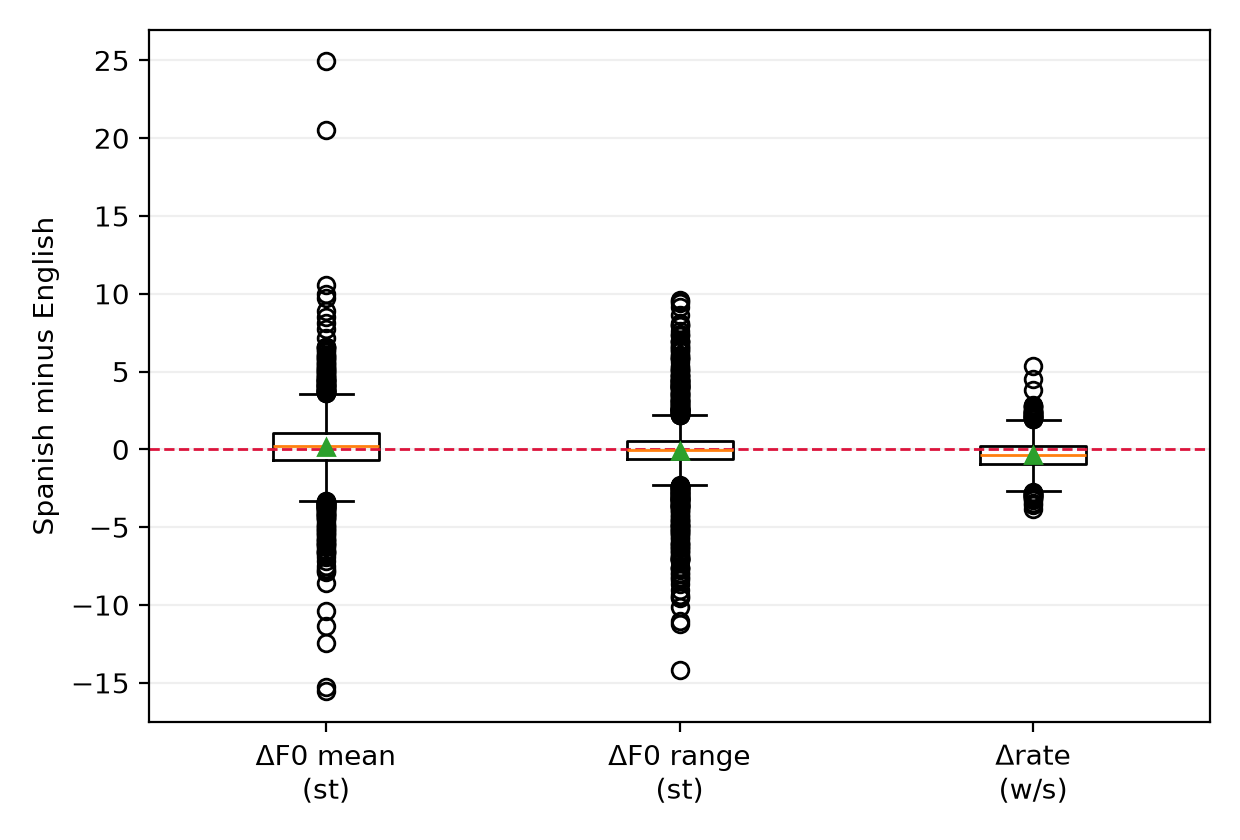
\includegraphics[width=0.78\linewidth]{figures/F_corpus_paired_deltas.png}
\caption{Distribution of paired Spanish-minus-English differences for each prosodic measure over
2{,}304 same-speaker pairs. The systematic language-level shifts reported in
Table~\ref{tab:corpusprosody} are small relative to the spread.}
\label{fig:paireddeltas}
\end{figure}

\begin{figure}[htbp]
\centering
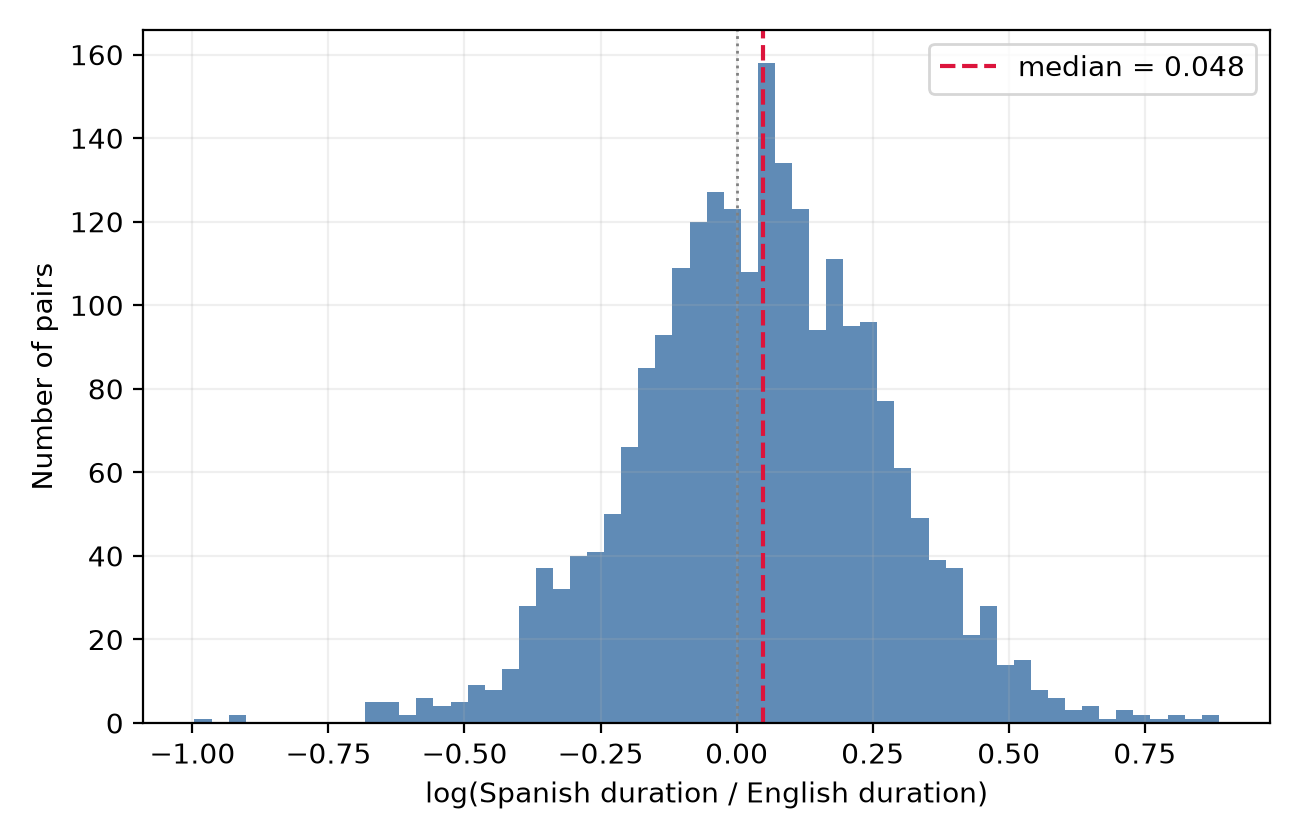
\includegraphics[width=0.78\linewidth]{figures/F_corpus_duration_ratio.png}
\caption{Log ratio of Spanish to English duration for the same speaker and the same content. The
median ratio of 1.049 is the human baseline against which the synthesiser's $1.52\times$ inflation
in Section~\ref{sec:duration_result} should be read.}
\label{fig:corpusdur}
\end{figure}

\begin{figure}[htbp]
\centering
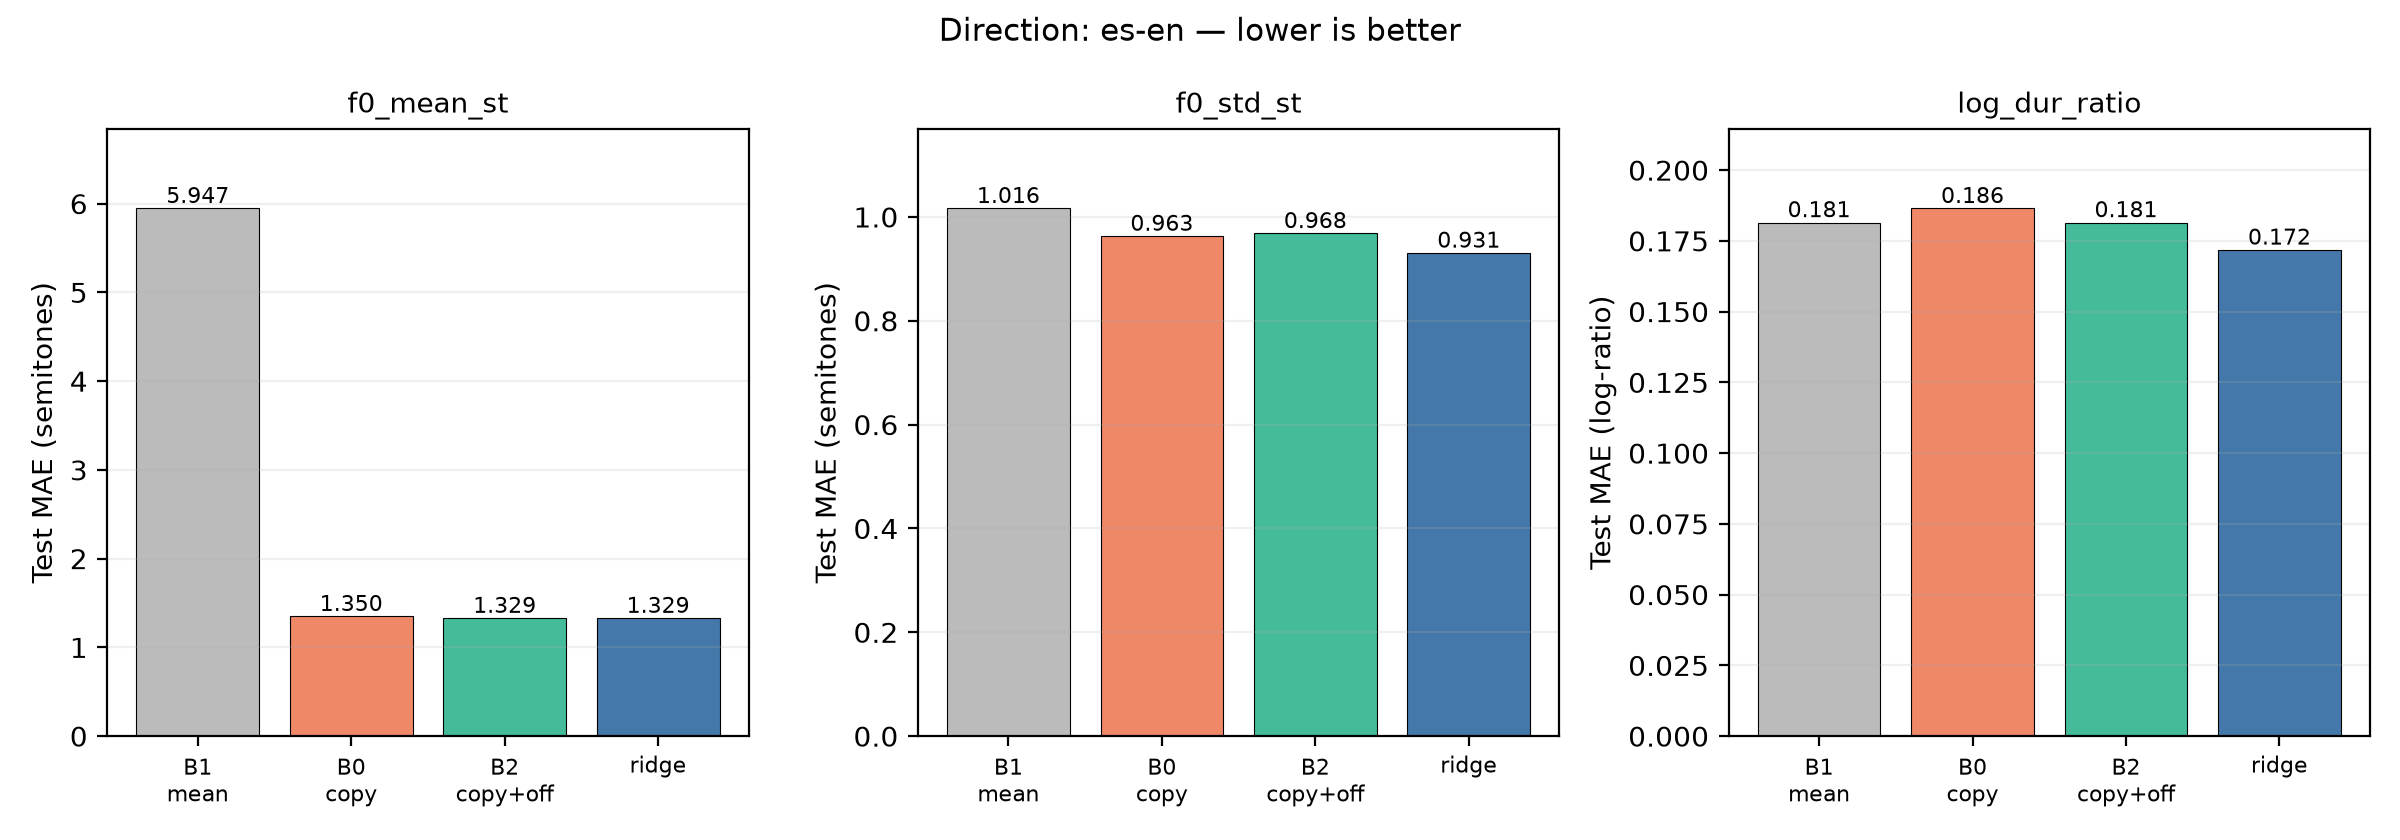
\includegraphics[width=0.86\linewidth]{figures/F_ridge_mae_es-en.png}
\caption{Test mean absolute error for each prosody target in the \esto{} direction, model against
the three baselines. The companion to Figure~\ref{fig:ridge}.}
\label{fig:ridgeesen}
\end{figure}

\begin{figure}[htbp]
\centering
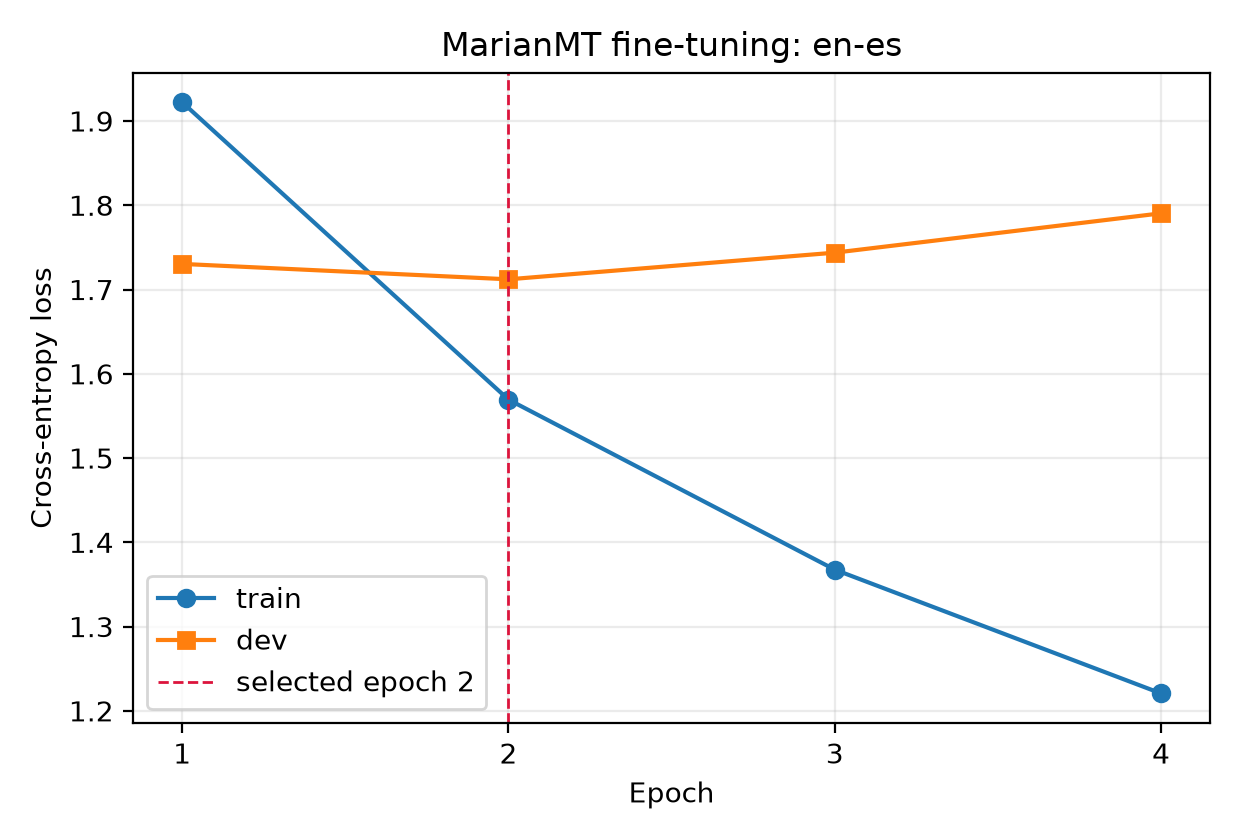
\includegraphics[width=0.86\linewidth]{figures/F_finetune_curves_en-es.png}
\caption{Training and development loss per epoch for \ento{} fine-tuning. Development loss is
minimised at epoch 2 and rises thereafter; the epoch-2 checkpoint was selected on that basis.}
\label{fig:ftcurveenes}
\end{figure}

\begin{figure}[htbp]
\centering
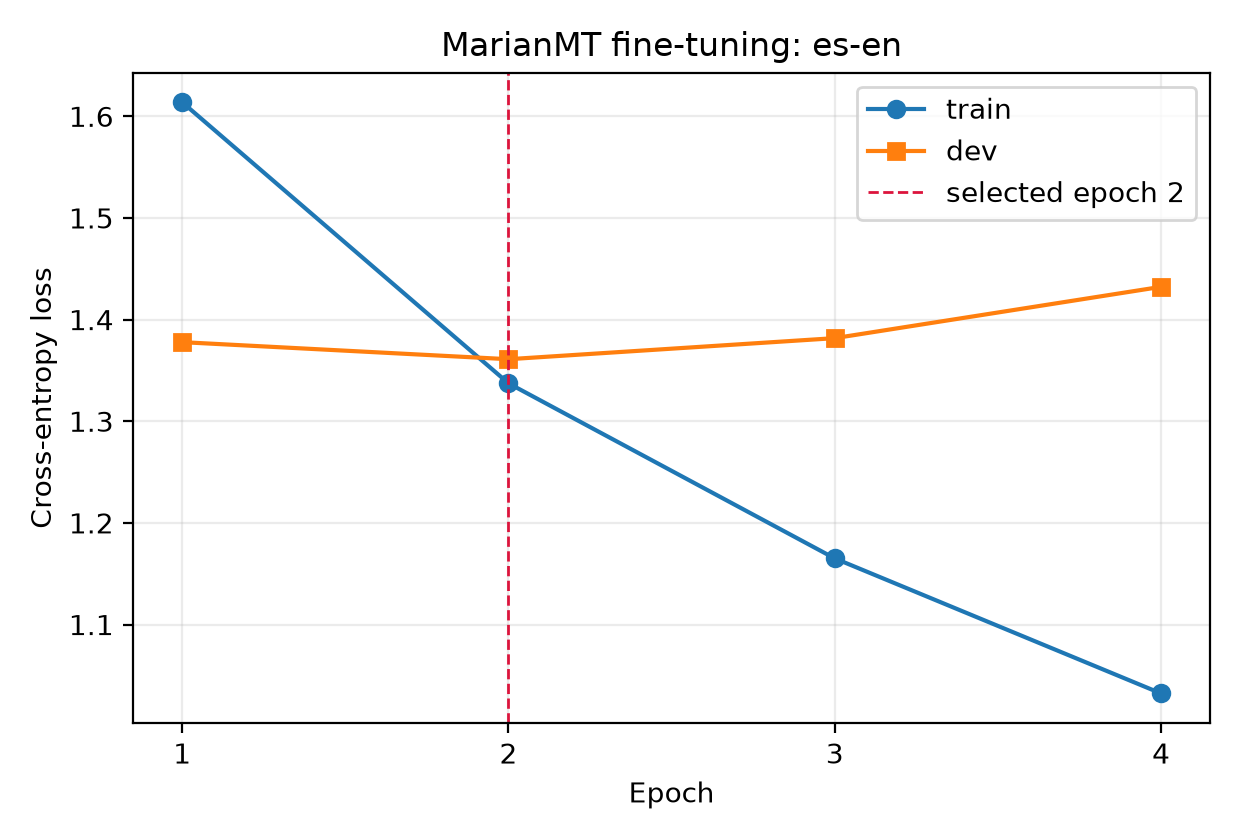
\includegraphics[width=0.86\linewidth]{figures/F_finetune_curves_es-en.png}
\caption{Training and development loss per epoch for \esto{} fine-tuning. The same epoch was
selected independently in this direction.}
\label{fig:ftcurveesen}
\end{figure}

% =======================================================================================
\chapter{Computational Environment and Provenance}
\label{app:provenance}

The record below is written automatically beside the analysis outputs each time the report is
generated, so that the figures in this dissertation can be tied to an exact state of the code.

\vspace{0.4\baselineskip}
{\singlespacing\small
\begin{tabular}{@{}ll@{}}
\toprule
\textbf{Item} & \textbf{Value} \\
\midrule
Git commit                & \texttt{ea7542c} \\
Python                    & 3.11.16 \\
Platform                  & macOS 26.6, arm64 (Apple silicon) \\
NumPy / pandas / SciPy    & 2.4.6 / 2.3.3 / 1.17.1 \\
librosa / matplotlib      & 0.11.0 / 3.11.1 \\
Random seed               & 498 (splits, fine-tuning, bootstrap) \\
F0 search band            & 65--1000\,Hz \\
F0 plausibility band      & 60--400\,Hz \\
Quality gate              & voiced ratio $\geq0.30$; duration 0.4--20\,s \\
Feature set               & \texttt{t1}: F0 level, F0 range, log duration, voiced ratio, \\
                          & \phantom{\texttt{t1}: } word count, speaking rate \\
Regularisation grid       & $10^{-3}$ to $10^{6}$, ten values \\
Recognition model         & Whisper \texttt{small} (CPU) \\
Translation models        & \pth{Helsinki-NLP/opus-mt-en-es}, \pth{opus-mt-es-en} \\
Synthesis model           & Coqui XTTS-v2 (CPU) \\
Speaker encoder           & \pth{speechbrain/spkrec-ecapa-voxceleb} (CPU) \\
Deep-learning framework   & PyTorch (no TensorFlow or Keras is used anywhere) \\
\bottomrule
\end{tabular}\par}

\vspace{0.6\baselineskip}
\noindent
Two components were adapted by the authors: the translation models, fine-tuned as described in
Section~\ref{sec:finetune_method}, and the ridge prosody model, which is a closed-form statistical
fit of six coefficients rather than a deep-learning model and is described as such throughout. The
recognition, synthesis and speaker-embedding models are used exactly as released.
